\documentclass[12pt]{article}
\usepackage[margin=3cm]{geometry}
\usepackage[portuguese]{babel}
\usepackage[utf8]{inputenc}
\usepackage{hyperref}
\usepackage{indentfirst}
\usepackage{subfig}

\urlstyle{same}
\pagenumbering{arabic}
%\usepackage{multicol}
\hypersetup{
    colorlinks=true,
    linkcolor=black,
    filecolor=magenta,      
    urlcolor=blue,
    citecolor=black,
}
\usepackage[backend=bibtex]{biblatex}
\usepackage{graphicx}
\pagestyle{plain}

\newcommand{\melita}{Diogo Melita, 99202}
\newcommand{\gaspar}{Diogo Gaspar, 99207}
\newcommand{\grupo}{al038}

\begin{document}
\begin{center}
{\Huge{Relatório 1º Projeto ASA 2021/2022}} \\
\vspace{0.5mm}
{\large{\melita \quad \gaspar}} \\
\vspace{0.5mm}
{\large{Grupo: \grupo}} \\
\end{center}

\section{Descrição do Problema e da Solução}
Foi proposta a resolução de dois problemas clássicos associados à programação dinâmica: o de, dada uma sequência de inteiros, indicar o comprimento da sua maior subsequência estritamente crescente, \textbf{LIS}, e respetiva quantidade, e o de, dadas duas sequências de inteiros, indicar o comprimento da maior subsequência comum estritamente crescente entre ambas, \textbf{LCIS}. 

\vspace{0.5mm}
Para solucionar o \textbf{primeiro problema}, recorreu-se ao \textit{patience sorting} [1] - a sua estrutura permite organizar os números em \textit{pilhas}, considerando cada número uma \textit{carta}. Cada carta é colocada na pilha mais à esquerda possível - pode colocar-se uma carta numa pilha caso a carta do topo da mesma tenha valor igual ou superior à da carta a inserir. São mantidas somas cumulativas em cada carta, correspondendo à LIS a terminar nela caso o algoritmo parasse aí. Finalizado o algoritmo, tem-se que o número de pilhas corresponde ao comprimento máximo da LIS, e que a soma cumulativa guardada na carta do topo da pilha mais à direita será o número de ocorrências dessa mesma LIS.

\vspace{0.5mm}
A solução para o \textbf{segundo problema} teve por base uma abordagem em programação dinâmica [2]. Recorreu-se a um vector, $l$, que, no final, terá em cada entrada o comprimento da LCIS a terminar no elemento correspondente da segunda sequência-argumento. Ambas as sequências são percorridas, e, para cada elemento: se os elementos forem \textbf{iguais} e a LCIS a ser formada com esse elemento comum for maior que a LCIS já conhecida a terminar nele, a entrada correspondente em $l$ é incrementada. Caso o elemento do primeiro vector for \textbf{maior} que o segundo e a LCIS a ser construída no ciclo atual for menor que a LCIS encontrada no elemento do segundo vector, então o comprimento da LCIS a ser construída é atualizado para esse valor. O valor máximo de $l$ corresponde ao comprimento da LCIS.

\section{Análise Teórica}
Seja $n$ o tamanho da primeira sequência e, no, caso do problema 2, $m$ o tamanho da segunda sequência.
O custo temporal e espacial da leitura dos dados de entrada para ambos os problemas é de $\Theta(n)$ e $\Theta(n + m)$, respetivamente. Para o primeiro problema, trata-se de uma simples leitura do input para um vector de inteiros, enquanto que para o segundo problema recorreu-se a uma abordagem diferente: os inteiros da primeira sequência são guardados num vector e num mapa, mapa esse com tempos de acesso e inserção $O(1)$, de modo a facilitar guardar apenas os elementos comuns entre as sequências ao ler a segunda sequência.

\vspace{0.5mm}

Para o \textbf{primeiro problema}, foram utilizados vectores de pilhas e de as somas cumulativas (inteiros). Existem exatamente $n$ cartas, pelo que a complexidade espacial de cada uma dessas estruturas é $\Theta(n)$. No total do algoritmo, portanto, o custo espacial fica em $\Theta(n)$ (contando, claro, com o tratamento do \textit{input} referido acima). O ciclo principal percorre todas as cartas, $\Theta(n)$, e por cada carta é necessário realizar duas pesquisas binárias, uma para saber em que pilha inserir a carta e outra para saber a soma cumulativa com que contar da pilha anterior, $O(2\log{n}) = O(\log{n})$. Assim sendo, a complexidade temporal total do algoritmo é de $O(n\log{n})$. A apresentação dos resultados é realizada em $O(1)$, já que obter o tamanho de um vector e o último elemento do mesmo são operações realizadas em tempo constante, não tendo influência na complexidade temporal do algoritmo.

\vspace{0.5mm}

Já em relação ao \textbf{segundo problema}, é guardado um vector com $m$ elementos, $\Theta(m)$. O custo espacial é, portanto, $\Theta(n + m)$, contando com o tratamento de dados. Todos os elementos da primeira sequência são comparados com todos os da segunda, ocorrendo, no pior caso, $O(nm)$ comparações. O algoritmo tem, portanto, complexidade temporal $O(nm)$. Para a apresentação dos dados, ocorre uma passagem linear, $O(m)$, por um vector, sem influência, portanto, na complexidade temporal do algoritmo.

\section{Avaliação Experimental dos Resultados}
Para analisar o algoritmo, optou-se por usar a ferramenta \texttt{hyperfine} para \textit{benchmarking}, gerando sequências de tamanho arbitrário com um pequeno programa em \texttt{Python} (sequências ordenadas de forma estritamente crescente).

\begin{figure}[h]
    \centering
    \subfloat[\centering Solução - Problema 1 ($O(n\log{n})$)]{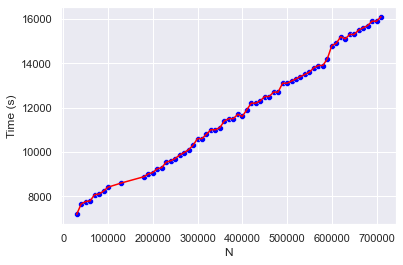
\includegraphics[width=7.35cm]{graph-problem-1.png}}
    \qquad
    \subfloat[\centering Solução - Problema 2 ($O(nm)$)]{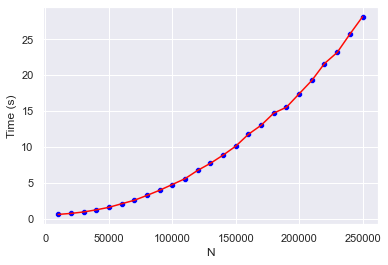
\includegraphics[width=7.35cm]{graph-problem-2.png}}
    \caption{Complexidade temporal da solução proposta para os dois problemas}
    \label{fig:graph-problem-1-2}
\end{figure}
\vspace{0.5mm}

Os valores obtidos demonstram, para o problema 1, uma tendência $n\log{n}$ na curva do gráfico, e uma $nm$ para o problema 2, tal como esperado. De realçar que para o problema 2 foi utilizado um valor de $m$ igual ao de $n$, por simplicidade.

\begin{thebibliography}{2}
    \bibitem{Problem1}
    Wayne, K. (2018, April 11). \textit{Longest Increasing Subsequence} [PowerPoint slides]. Computer Science Department, Princeton University.

    \bibitem{Problem2}
    Sakai, Y. (2006). \textit{A linear space algorithm for computing a longest common increasing subsequence}.
\end{thebibliography}

\end{document}